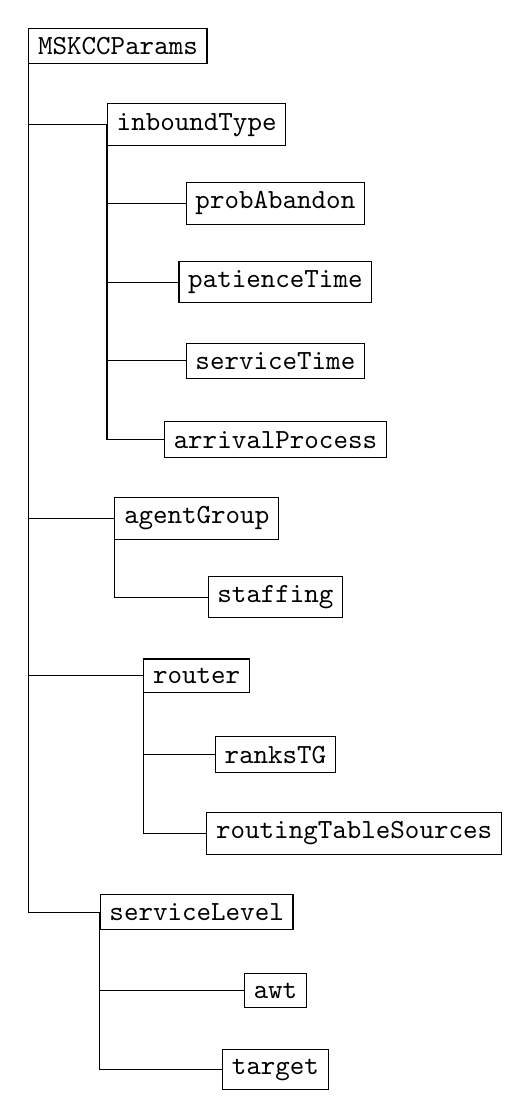
\begin{tikzpicture}[shape=rectangle,anchor=west]
\node (MSKCCParams) [draw] {\texttt{MSKCCParams}};
\node (inboundType) [draw, below of=MSKCCParams, xshift=1cm]
{\texttt{inboundType}};
\node (probAbandon) [draw, below of=inboundType, xshift=1cm]
{\texttt{probAbandon}};
\node (patienceTime) [draw, below of=probAbandon]
{\texttt{patienceTime}};
\node (serviceTime) [draw, below of=patienceTime]
{\texttt{serviceTime}};
\node (arrivalProcess) [draw, below of=serviceTime]
{\texttt{arrivalProcess}};
\node (agentGroup) [draw, below of=arrivalProcess, xshift=-1cm]
{\texttt{agentGroup}};
\node (staffing) [draw, below of=agentGroup, xshift=1cm]
{\texttt{staffing}};
\node (router) [draw, below of=staffing, xshift=-1cm]
{\texttt{router}};
\node (ranksTG) [draw, below of=router, xshift=1cm]
{\texttt{ranksTG}};
\node (routingTableSources) [draw, below of=ranksTG, xshift=1cm]
{\texttt{routingTableSources}};
\node (serviceLevel) [draw, below of=routingTableSources, xshift=-2cm]
{\texttt{serviceLevel}};
\node (awt) [draw, below of=serviceLevel, xshift=1cm]
{\texttt{awt}};
\node (target) [draw, below of=awt]
{\texttt{target}};

\draw (MSKCCParams.west) |- (inboundType)
(MSKCCParams.west) |- (agentGroup)
(MSKCCParams.west) |- (router)
(MSKCCParams.west) |- (serviceLevel);
\draw (inboundType.west) |- (probAbandon)
(inboundType.west) |- (patienceTime)
(inboundType.west) |- (serviceTime)
(inboundType.west) |- (arrivalProcess);
\draw (agentGroup.west) |- (staffing);
\draw (router.west) |- (ranksTG)
(router.west) |- (routingTableSources);
\draw (serviceLevel.west) |- (awt)
(serviceLevel.west) |- (target);
\end{tikzpicture}
